% Niveau :      PCSI *
% Discipline :  Chimie Orga
% Mots clés :   Stéréochimie

\begin{exercise}{Modèle clé-serrure de Michaelis--Menten}{3}{PCSI}
{Transformationn de la matière,Cinétique,Arrhénius}{bermu}

\begin{questions}
\questioncours Profil d'énergie potentielle d'une réaction chimique et influence d'un catalyseur.

\begin{EnvUplevel}
     En 1913, à partir de résultats expérimentaux, Victor Henri, Leonor Michaelis et Laure Menten proposent pour une réaction enzymatique
     $$\mathrm{\underset{\text{substrat}}{S} \overset{E}{=} \underset{\text{produit}}{P}},$$
     le mécanisme clé-serrure suivant :
     \begin{figure}[H]
         \centering
         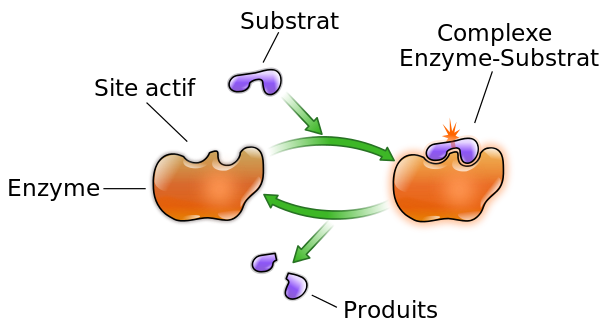
\includegraphics[width=0.6\linewidth]{gene/michaelis.png}
         \caption{Mécanisme clé-serrure}
         \label{fig:my_label}
     \end{figure}
     
     On notera [E$^\ast$] la concentration du complexe enzyme-substrat, [E] la concentration d'enzyme, [S] la concentration du substrat et [P] la concentration du produit.
     
\end{EnvUplevel}

\question En vous inspirant de la Figure 1, proposer un mécanisme en deux étapes modélisant la réaction. \\ On considérera que les deux étapes, notées 1 et 2, sont élémentaires, réversibles et de constantes $k_1$, $k_{-1}$ et $k_2$, $k_{-2}$.

\question Caractériser l'équilibre de la réaction S = P.

\question En notant $v(t)$ la vitesse de production de P, donner la loi de vitesse dans l'AEQS en fonction des concentrations [S]$_t$ et [P]$_t$, de la concentration totale en enzyme [E]$_\text{tot}$ = [E]$_t$ + [E$^\ast$]$_t$ et des constantes cinétiques.

\paragraph{Aide :} on pourra chercher la valeur de $\dfrac{[\text{E}^\ast]}{[\text{E}]}$ dans le cadre de l'AEQS et en déduire $\dfrac{[\text{E}]}{[\text{E}]_\text{tot}}$ et  $\dfrac{[\text{E}^\ast]}{[\text{E}]_\text{tot}}$.

\question \'Evaluer les vitesses maximales dans le sens S $\rightarrow$ P et P $\rightarrow$ S.

\question En déduire que la loi de vitesse peut s'écrire
$$v(t) = \dfrac{k_1 v^\text{max}_{\text{S} \rightarrow \text{P}}[\text{S}] - k_{-2} v^\text{max}_{\text{P} \rightarrow \text{S}}[\text{P}]}{k_1(c_\text{s} + [\text{S}]) + k_{-2}(c_\text{p} + [\text{P}])},$$
où $c_\text{s}$ et $c_\text{p}$ sont les deux constantes dites de Michaelis dont on donnera les expressions.

Donner un sens chimique à cette expression.

\uplevel{On se place désormais dans le cas où l'étape donnant le produit est perçue comme irréversible.}

\question Interpréter chimiquement ce que cela signifie à partir de la loi de vitesse de la question 4 et de la constante d'équilibre de la question 3.

\question En déduire une expression simplifiée de la loi de vitesse de la question 6, dépendant uniquement de $v^\text{max}_{\text{S} \rightarrow \text{P}}$ et $c_\text{s}/[\text{S}]$.

\question Etablir une méthode graphique pour évaluer $v_\text{max}$ et $c_\text{s}$.

\end{questions}

\end{exercise}